\subsection{Подробный разбор выбранного подхода?!}
    Надо подумать куда это лучше поместить

        Обоснование почему был выбран WTMF-G;

        tfidf в качестве baseline

    \subsubsection{Построение датасетов}
        За один и тот же промежуток выкачиваем твиты с помощью stream api, новости с помощью rss.

        Твит задаётся кортежем: (time, author, text). Новость задаётся кортежем: (time, title, summary, url).

        Train/test множества формируем из твитов, которые содержат единственную ссылку на новость, из выкаченных нами ранее, и не совпадают с заголовком новости.

    \subsubsection{WTMF}
        WTMF - модель применяемая для анализа схожести между короткими текстами \cite{wtmf}. Модель рассматривает отсутствующие в тексте слова как признаки короткого текста. Отсутсвующие слова это все слова корпуса рассматриваемых текстов за исключением слов из рассматриваемого короткого текста. Отсутствующие слова являются негативным сигналом для смысла коротких текстов.

        WTMF похож на SVD, но использует не разложение, а непосредственный расчёт каждой ячейки. Модель раскладывает матрицу $X \sim P^TQ$.

        Корпус рассматривается как матрица $X$ размера $M \times N$: строки - это слова (всего $M$), столбцы - короткие тексты (всего $N$), ячейки - мера tf-idf.
        Как показано на рисунке~\ref{pic:wtmf} матрица $X$ приближается произведением двух матриц $P$ размера $M \times K$ и $Q$ размера $K \times N$.

        \begin{figure}[h!]
            \center
            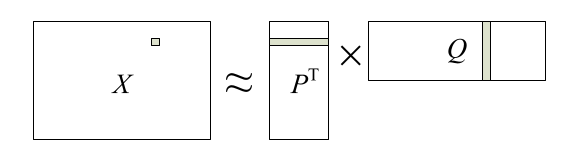
\includegraphics[scale=0.45]{wtmf.png}
            \caption{wtmf}
            \label{pic:wtmf}
        \end{figure}

        Каждый текст $s_j$ представлен в виде вектора $Q_{\cdot,j}$ размерности $K$, каждое слово $w_i$ представлено в виде вектор $P_{i,\cdot}$. Когда их скалярное произведение $X_{ij}$ близко к нулю, то мы считаем, что это отсутствующее слово.

        Задачей модели является минимизация целевой функции ({\color{red}$\lambda$ - регуляризирующий член}, матрица W определяет вес каждого элемента матрицы X):
        $$\sum_i \sum_j W_{ij} (P_{i,\cdot} \cdot Q_{\cdot,j} - X_{ij})^2 + \lambda ||P||^2_2 + \lambda ||Q||^2_2.$$

        Для получения векторов $P_{i,\cdot}$ и $Q_{\cdot,j}$ используется алгоритм описанный в статье~\cite{matrix_approximation}. Сначала P и Q инициализируются случайными числами. Затем запускается итеративный пересчёт P и Q по следующим формулам (эффективный способ расчёта описан в \cite{steck_recommender}):
        $$P_{i, \cdot} = (Q W'_i Q^T + \lambda I)^{-1} Q W'_i X_{i,\cdot}^T,$$
        $$Q_{\cdot, j} = (P W'_j P^T + \lambda I)^{-1} P W'_j X_{j,\cdot}.$$
        Здесь $W'_i = diag(W_{i, \cdot})$ - диагональная матрица полученная из $i$-ой строчки матрицы $W$, аналогично $W'_j = diag(W_{\cdot, j})$ - диагональная матрица полученная из $j$-ого столбца.

        Определим матрицу W следующим образом:
        \begin{gather}
            W_{ij} =
            \begin{cases}
                1, ~~if~X_{ij} \neq 0, \nonumber \\
                w_m, ~~otherwise.
            \end{cases},
        \end{gather}
        где $w_m$ положительно и $w_m << 1$.

    \subsubsection{Построение связей текст-текст}
        Твиты связываются с помощью хэштегов, named entities и времени.

        Связь твитов с помощью хэштэгов. Сначала извлекаем все хэштеги из твитов, затем превращаем в хэштеги все слова во всех твитах, которые совпали с ранее извлечёнными хэштэгами. Для каждого твита и для каждого хэштэга извлекаем $k$ твитов, которые содержат этот этот хэштег, если хэштег появлялся в более чем $k$ твитах берём $k$ твитов наиболее близких во времени к исходному.

        Связь твитов с помощью named entities. Применяем методы NER к новостным summary и получаем множество named entities. Затем применяем тот же подход, что и к хэштегам, сначала превращаем в NE слова из твитов, которые совпали с полученными NE, а затем получаем $k$ связей для каждого твита.

        Связь твитов с помощью времени. Аналогично вышеописанному для каждого твита выбираем $k$ связей с наиболее схожими твитами в окрестности 24 часов. Наиболее близкие находятся с помощью косинусной меры, расчитываемой для векторов из таблицы X.

        Новости связываются только по времени.
    \subsubsection{WTMF-G}
        Добавление связей текст-текст в WTMF происходит с помощью влияния на regularization term. Для каждой пары связанных текстов $j_1$ и $j_2$:
        $$\lambda = \delta \cdot (\dfrac{Q_{\cdot,j_1}\cdot Q_{\cdot,j_2}}{|Q_{\cdot,j_1}|| Q_{\cdot,j_2}|}-1)^2,$$
        коэффициент $\delta$ задаёт степень влияния связей текст-текст.

        Полученная модель и называется WTMF-G (WTMG on graphs).

        Alternating Least Square используемый в \cite{steck_recommender} не применим из-за нового regularization term, который зависит от $|Q_{\cdot,j}|$ ({\color{red} по-хорошему нужно понять почему}). Для того, чтобы мы могли применить ALS мы вводим упрощение: длина вектора $Q_{\cdot,j}$ не изменяется во время итерации. Получаем уравнения:
        $$P_{i, \cdot} = (Q W'_i Q^T + \lambda I)^{-1} Q W'_i X_{i,\cdot}^T,$$
        $$Q_{\cdot, j} = (P W'_j P^T + \lambda I + \delta  L_j^2 Q_{\cdot,n(j)} diag(L^2_{n(j)})Q_{\cdot,n(j)}^T)^{-1}   (P W'_j X_{j,\cdot} + \delta  L_j Q_{\cdot,n(j)} L_{n(j)}).$$
        В этих формулах $n(j)$~---~список связанных текстов с текстом $j$. $Q_{\cdot,n(j)}$~---~матрица, состоящая из связанных векторов для $Q_{\cdot, j}$. $L_j$ - длина вектора $Q_j$ на начало итерации, $L_n(j)$~---~вектор длин векторов связанных с $j$ i.e. $Q_{\cdot,n(j)}$, полученный на начало итерации.
